%
% File: chap_4.tex
% Author: Yuil Tripathee
%
\chapter{Systems Analysis and Design}

\section{Software Analysis}

\subsection{Class Diagram}

The rational behind this implementation is to have fastest and the most iterable base for our back-end. It blends the OOAD concept to adapt with relational design that is readily deployed on PostgreSQL database.

Figure ~\ref{fig:class} is the class diagram in our current system. The full image is available in the documentation repository, submitted along this project.

\begin{figure}[!h]
	\centering
	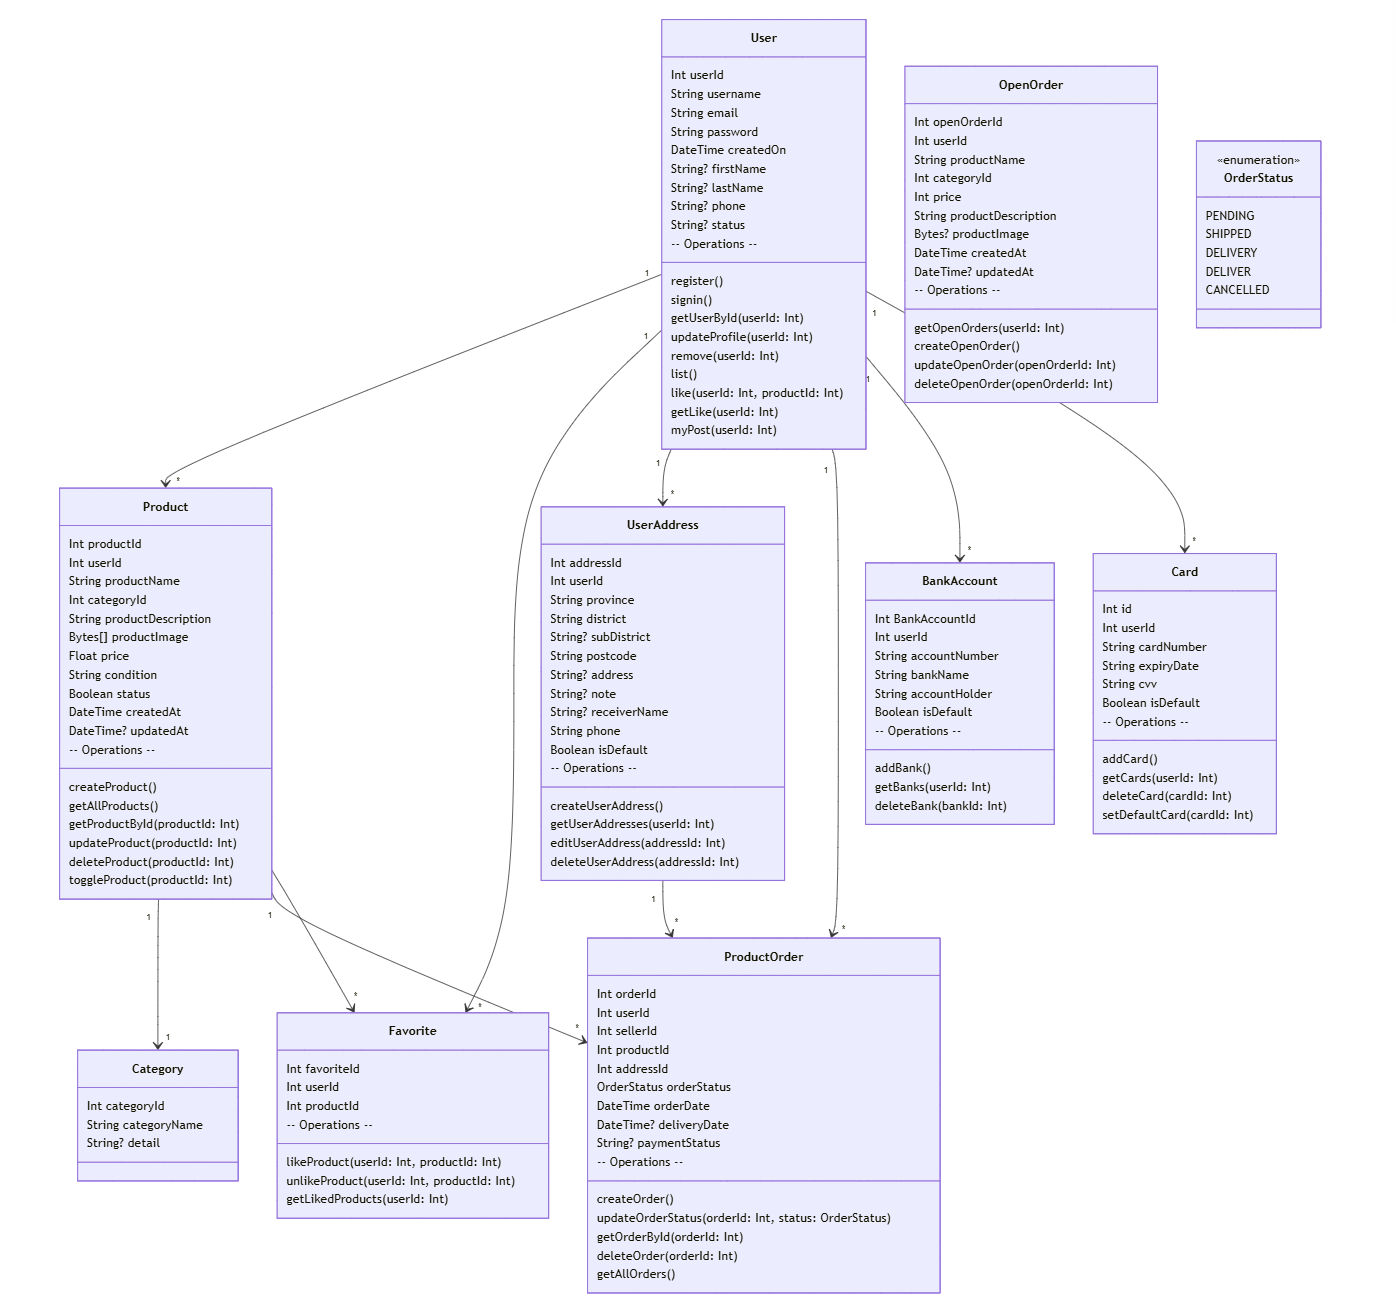
\includegraphics[width=1.1\textwidth]{chapters/ch-04/class.png} % Adjust width as needed
	\caption{Class Diagram}
	\label{fig:class} % Label for referencing the figure
\end{figure}

\subsection{Sequence Diagram}

The rational behind our sequence diagram is simple. We want to visualize and communicate how every machine components interacts in terms of interaction and data transfer in sequence of individual operations.

% TODO: paste a lot of sequence diagrams

\begin{figure}[!h]
	\centering
	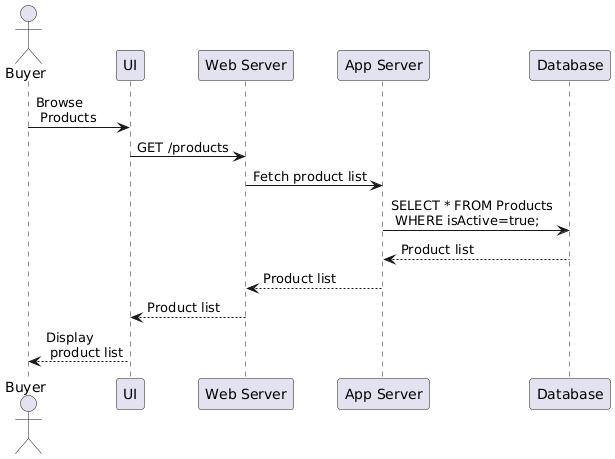
\includegraphics[width=0.9\textwidth]{chapters/ch-04/300_usecase_browse.png} % Adjust width as needed
	\caption{Sequence diagram for Use-case: Browse Products}
	\label{fig:seq_01} % Label for referencing the figure
\end{figure}

\begin{figure}[!h]
	\centering
	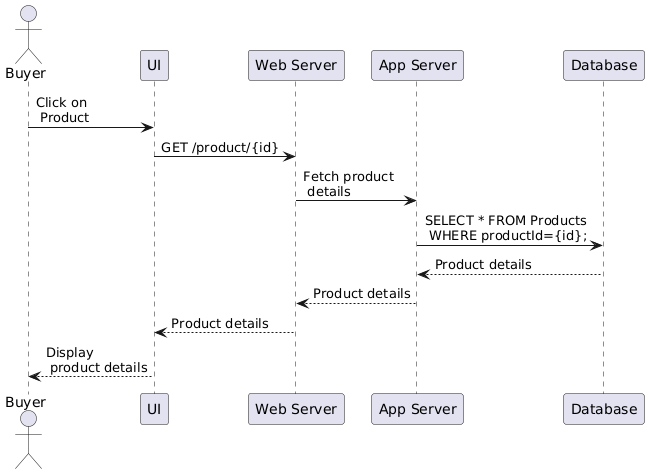
\includegraphics[width=0.9\textwidth]{chapters/ch-04/301_usecase_view.png} % Adjust width as needed
	\caption{Sequence diagram for Use-case: View Products}
	\label{fig:seq_02} % Label for referencing the figure
\end{figure}

\begin{figure}[!h]
	\centering
	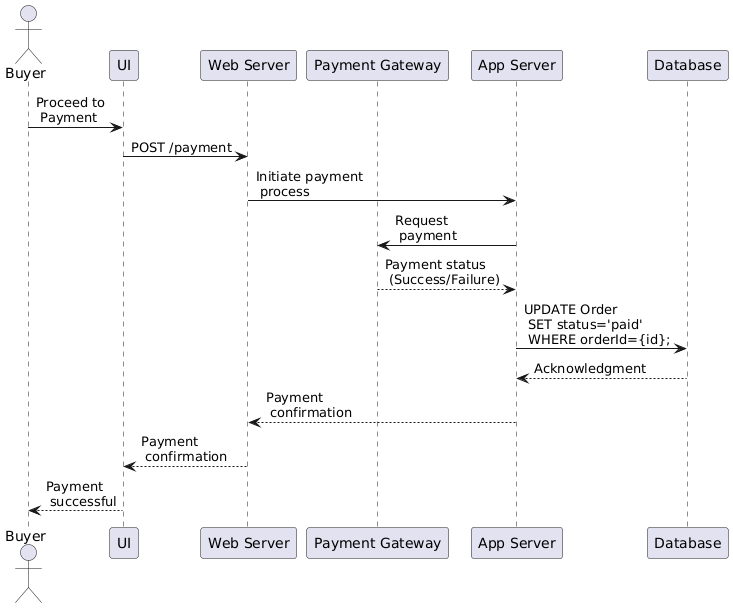
\includegraphics[width=1\textwidth]{chapters/ch-04/302_usecase_pay.png} % Adjust width as needed
	\caption{Sequence diagram for Use-case: Pay}
	\label{fig:seq_03} % Label for referencing the figure
\end{figure}

\begin{figure}[!h]
	\centering
	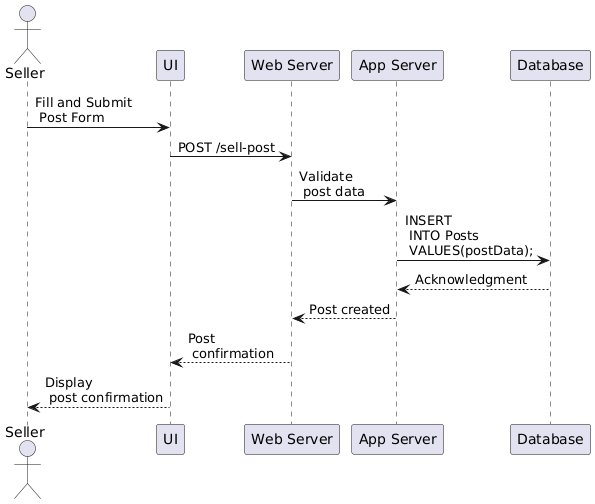
\includegraphics[width=0.8\textwidth]{chapters/ch-04/303_usecase_post.png} % Adjust width as needed
	\caption{Sequence diagram for Use-case: Post new products}
	\label{fig:seq_04} % Label for referencing the figure
\end{figure}

\begin{figure}[!h]
	\centering
	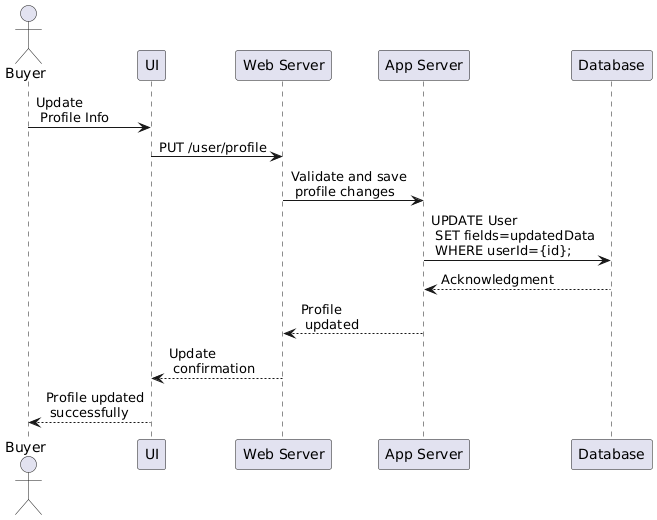
\includegraphics[width=0.9\textwidth]{chapters/ch-04/304_usecase_edit_profile.png} % Adjust width as needed
	\caption{Sequence diagram for Use-case: Edit profile}
	\label{fig:seq_05} % Label for referencing the figure
\end{figure}

\begin{figure}[!h]
	\centering
	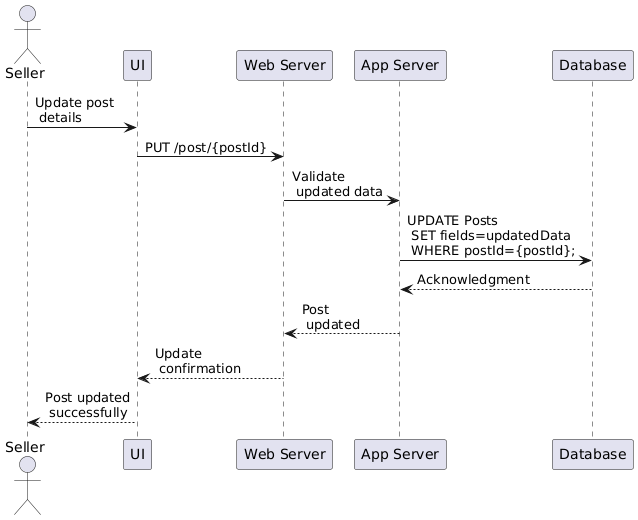
\includegraphics[width=0.9\textwidth]{chapters/ch-04/305_usecase_edit_post.png} % Adjust width as needed
	\caption{Sequence diagram for Use-case: Edit product post}
	\label{fig:seq_06} % Label for referencing the figure
\end{figure}

\subsubsection{Limitations}

\begin{description}
	\item[Unconventional implementation:] Coding syntax such as including SQL as part of modeling app sequences. This is not part of best practice as specified in the UML specifications. However, it serves us more effectively as the means of communication for different technical sub-teams (front end, back-end and the deployment team). Our rationale behind this was to address the knowledge gap our current development team has. For the further updates, we intend to move up to the standard specification as knowledge gap is shortened and the back-end team is ready to receive requirements inputs using the top level description.
	\item[Less flexibility to stack changes] For the current timeline, we chose the back-end stack to adapt customer needs as quickly as possible. However, if the requirements changes results in change of technical stack (for example, we switch from HTTP REST \& SQL interface to GraphQL \&gRPC); our specification for interaction sequences will be obsolete. The SQL-inspired specification cannot address changes to other modern day No-SQL schema (such as document store, column store). Therefore, if we change the database structure the specifics in the sequence diagram regarding SQL interface should be changed.
\end{description}

\section{Systems Design}

% Define goals of project
% Systems Design -> decompose to smaller sub-systems
% Object Design -> define domain (object, interface, ...)

\subsection{Demonstration model}

\begin{figure}[!h]
	\centering
	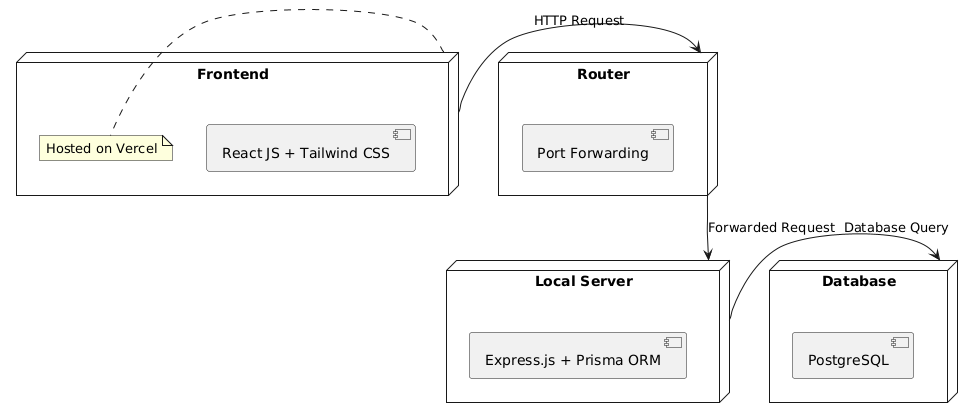
\includegraphics[width=0.9\textwidth]{chapters/ch-04/401_deploy_local.png} % Adjust width as needed
	\caption{Development phase components layout}
	\label{fig:deploy_1} % Label for referencing the figure
\end{figure}

Figure ~\ref{fig:deploy_1} is a minimal base on how our system is deployed and serving the user currently. We estimate to handle the peak of 10000 transactions per month comfortably in this setup. However, it might not meet the high up-time requirements as this server is currently hosted on our residential premises.

\subsection{Full scale production model}

\begin{figure}[!h]
	\centering
	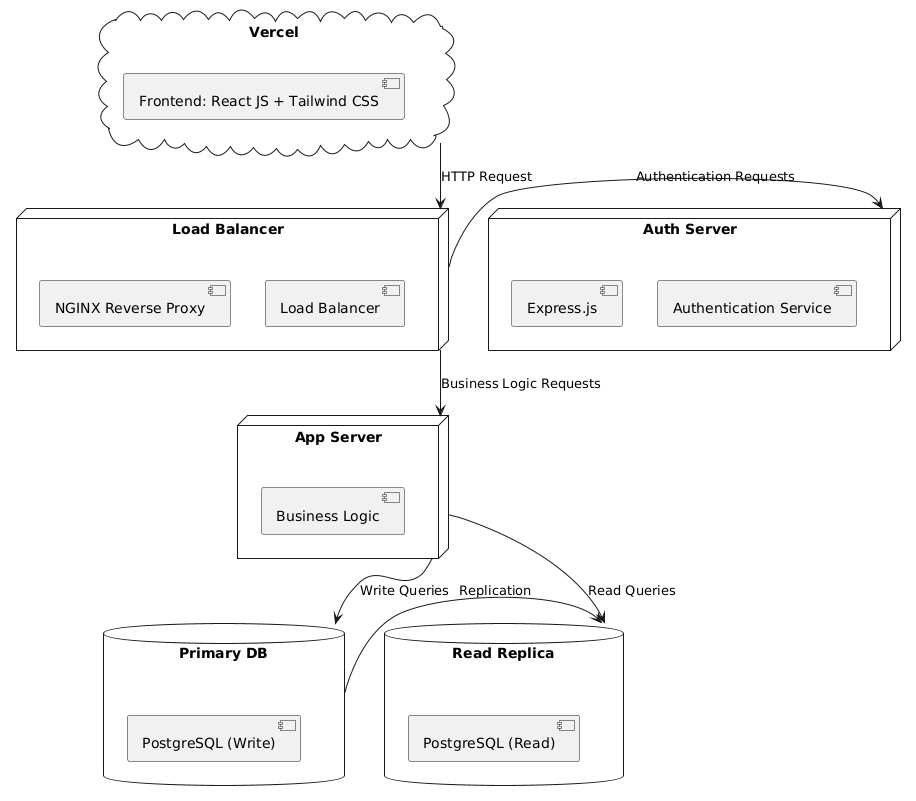
\includegraphics[width=1\textwidth]{chapters/ch-04/402_deploy_cloud.png} % Adjust width as needed
	\caption{Deployment phase components layout}
	\label{fig:deploy_2} % Label for referencing the figure
\end{figure}


Upon reaching the designated transaction volume, we intend to migrate our application to a dedicated cloud service. Figure ~\ref{fig:deploy_2} suggests the tentative plan that allows us to deploy in cloud and scale.

\clearpage